\documentclass[12pt]{article}

\usepackage{sbc-template}
\usepackage{float} % Para permitir o uso de [H]
 \usepackage{amsmath}
\usepackage{graphicx,url}
\usepackage{svg}
%\usepackage[brazil]{babel}   
\usepackage[utf8]{inputenc}  
\usepackage{authblk} 
\sloppy

\title{Relatório do Trabalho Final de Inteligência Artificial}

\author{Carlos Andres\inst{1}, Davi Carvalho\inst{1}, Gabriel Toyoda\inst{1}, Pedro Larry\inst{1}}

\address{Faculdade de Tecnologia -- Universidade Federal do Amazonas (UFAM)\\
   69080-900 -- Manaus -- AM -- Brazil
    \email{\{carlos.junior, davi.carvalho, gabriel.toyoda, pedro.lopes\}@icomp.ufam.edu.br}
}

\begin{document} 

\maketitle

\begin{abstract}
  This paper explores the application of artificial intelligence to solve the Michalski train problem, aiming to classify trains as going east or west based on their characteristics. To do this, different models are implemented and compared, including neural networks and a neuro-symbolic approach. Neural networks enable hierarchical learning of complex data representations, while the neuro-symbolic approach integrates symbolic techniques and neural networks, providing a more complete solution.
\end{abstract}
     
\begin{resumo} 
  Este artigo explora a aplicação de inteligência artificial para solucionar o problema do trem de Michalski, visando classificar trens como indo para leste ou oeste a partir de suas características. Para isso, diferentes modelos são implementados e comparados, incluindo redes neurais e uma abordagem neuro-simbólica. As redes neurais possibilitam a aprendizagem hierárquica de representações complexas dos dados, enquanto a abordagem neuro-simbólica integra técnicas simbólicas e redes neurais, proporcionando uma solução mais completa.
\end{resumo}


\section{Inteligência Artificial: Paradigmas Simbólico e Conexionista}

A inteligência artificial (IA) busca replicar a capacidade humana de raciocínio e aprendizado em sistemas computacionais.  Ao longo de sua história, a IA se desenvolveu em torno de dois paradigmas principais: o simbólico e o conexionista \cite{russell2003artificial}. O paradigma simbólico,  fundamentado na lógica e em representações explícitas do conhecimento,  se destaca pela capacidade de realizar inferências complexas e lidar com raciocínio simbólico,  sendo fundamental em áreas como planejamento e resolução de problemas \cite{haugeland1989artificial}. Por outro lado, o paradigma conexionista,  inspirado no funcionamento do cérebro humano,  utiliza redes neurais artificiais para aprender padrões complexos a partir de dados,  demonstrando grande eficácia em tarefas como reconhecimento de padrões e processamento de linguagem natural \cite{haykin2009neural}.

\subsection{Redes Neurais Artificiais: Modelando o Cérebro}

Redes neurais artificiais (RNAs) são modelos computacionais inspirados na estrutura e função do cérebro humano \cite{kohonen2012self}.  Elas consistem em unidades básicas de processamento,  os neurônios artificiais,  organizados em camadas interconectadas. Cada conexão entre neurônios possui um peso associado,  que determina a influência da ativação de um neurônio sobre outro. O aprendizado em uma RNA se dá através do ajuste iterativo desses pesos,  permitindo que a rede modifique seu comportamento em resposta aos dados de treinamento \cite{hinton2006reducing}.

\begin{figure}[h!]
\centering
\includesvg[width=0.6\textwidth]{rede_neural.svg}
\caption{Exemplo de Rede Neural Artificial com múltiplas camadas ocultas.}
\label{fig:rede_neural}
\end{figure}

Uma característica crucial das RNAs é a capacidade de aprender representações hierárquicas dos dados de entrada \cite{bengio2009learning}.  Através de múltiplas camadas de processamento,  a rede aprende a extrair features cada vez mais abstratas e complexas,  construindo representações sofisticadas que capturam as relações intrínsecas presentes nos dados. Essa capacidade de aprendizado hierárquico torna as RNAs ferramentas poderosas para lidar com problemas complexos,  envolvendo grandes quantidades de dados,  como reconhecimento de imagens \cite{krizhevsky2012imagenet},  processamento de linguagem natural \cite{collobert2008unified} e previsão de séries temporais \cite{hochreiter1997long}.

\subsection{Aprendizagem Neuro-Simbólica: Em Busca da Sinergia entre Símbolos e Conexões}

Apesar do sucesso em diversas áreas, as RNAs tradicionais também apresentam desafios.  Um dos principais desafios reside na opacidade da representação do conhecimento. Os pesos ajustados durante o treinamento codificam o conhecimento adquirido pela rede,  mas essa codificação geralmente é distribuída e opaca,  dificultando a interpretação e explicação do comportamento do modelo por parte dos humanos \cite{lipton2018mythos}.  Essa falta de transparência pode ser um obstáculo em áreas onde a compreensibilidade do modelo é crucial,  como saúde e justiça criminal,  onde a explicabilidade das decisões tomadas por sistemas de IA é fundamental \cite{doshi2017towards}.

Além disso,  RNAs tradicionais enfrentam dificuldades em lidar com tarefas que exigem raciocínio simbólico e manipulação de conhecimento estruturado,  habilidades inerentes à cognição humana.  Sistemas simbólicos,  como os baseados em lógica de primeira ordem,  excelem nesse tipo de tarefa,  mas geralmente têm dificuldades em lidar com a incerteza inerente a muitos problemas do mundo real e com a necessidade de generalizar a partir de grandes conjuntos de dados \cite{besold2017neural}.

A aprendizagem neuro-simbólica (ANS) surge como uma área de pesquisa promissora que busca combinar as vantagens das abordagens conexionistas e simbólicas \cite{garcez2002neural}.  Em vez de tratá-las como mutuamente exclusivas,  a ANS visa integrá-las,  criando sistemas híbridos que combinam a capacidade de aprendizado de máquina das RNAs com a capacidade de raciocínio simbólico dos sistemas baseados em lógica.  Essa integração busca criar sistemas de IA mais robustos,  flexíveis e capazes de lidar com uma gama maior de tarefas,  incluindo aquelas que exigem tanto aprendizado a partir de dados quanto raciocínio simbólico \cite{bottou2017geometric}.

Diversas abordagens têm sido exploradas dentro da ANS,  incluindo:

\begin{itemize}
\item \textbf{Injeção de Conhecimento:} Nesta abordagem,  o conhecimento simbólico,  na forma de regras lógicas,  restrições ou conhecimento prévio do domínio,  é incorporado na estrutura da rede neural ou no seu processo de treinamento  \cite{hu2018harnessing}.   Essa integração pode se dar através da inicialização dos pesos da rede com base em regras lógicas,  da adição de termos regulares à função de perda que incentivam a conformidade com o conhecimento simbólico,  ou mesmo da modificação da própria arquitetura da rede para refletir as relações simbólicas presentes no domínio do problema.
\item \textbf{Extração de Regras:}  Após o treinamento de uma rede neural,  técnicas de extração de regras são aplicadas para traduzir o conhecimento aprendido pela rede,  expresso implicitamente nos pesos das conexões,  em regras lógicas ou outras formas de representação simbólica,  tornando o conhecimento adquirido pela rede mais compreensível para humanos \cite{haykin2009neural}. Essas regras podem ser utilizadas para diversas finalidades,  como  a validação do modelo,  a identificação de novas relações nos dados ou a criação de sistemas especialistas baseados em regras.
\item \textbf{Arquiteturas Híbridas:} Sistemas híbridos combinam módulos neurais e simbólicos em uma arquitetura única e coesa \cite{serafini2016logic}. Esses módulos interagem entre si,  permitindo a troca de informações e a resolução conjunta de problemas. Um exemplo clássico é a arquitetura Connectionist Modal Logic (CML) proposta por Garcez et al. (2007),  que integra redes neurais com lógica modal para representar e raciocinar sobre conhecimento relacional. 
\end{itemize}

A escolha da abordagem mais adequada para a integração neuro-simbólica depende da natureza do problema,  dos dados disponíveis,  dos objetivos da aplicação e dos recursos computacionais disponíveis.

\section{Fundamentos Teóricos da Aprendizagem Neuro-Simbólica}

A aprendizagem neuro-simbólica (ANS)  representa uma área de pesquisa vibrante e promissora dentro da inteligência artificial.  Seu objetivo principal é a criação de sistemas que combinam as capacidades de aprendizado de máquina de sistemas conexionistas,  como as redes neurais,  com as capacidades de representação do conhecimento e raciocínio lógico de sistemas simbólicos \cite{garcez2009neural}. Essa integração visa superar as limitações inerentes a cada paradigma,  criando sistemas mais robustos,  interpretáveis e eficientes \cite{besold2017neural}.

\subsection{Motivações para a Hibridização Neuro-Simbólica}

A busca pela integração neuro-simbólica é motivada pelas limitações dos paradigmas simbólico e conexionista quando considerados isoladamente.

\begin{itemize}
\item \textbf{Opacidade das Redes Neurais:} Redes neurais,  apesar de eficazes em diversas tarefas,  geralmente atuam como "caixas pretas",  dificultando a compreensão humana do processo de tomada de decisão \cite{castelvecchi2016can}.  A falta de interpretabilidade limita a confiança e a aplicabilidade dessas redes em domínios críticos,  como saúde e finanças,  onde a explicabilidade e justificativa das decisões são cruciais \cite{guidotti2018survey}.
\item \textbf{Limitações dos Sistemas Simbólicos:} Sistemas simbólicos,  por outro lado,  oferecem transparência e explicabilidade,  mas enfrentam desafios em lidar com dados ruidosos,  incerteza e aprendizado a partir de grandes conjuntos de dados,  cenários onde as redes neurais se destacam \cite{smolensky1988connectionist}.  A manipulação simbólica também pode ser computacionalmente cara em cenários complexos,  limitando a escalabilidade desses sistemas.
\end{itemize}

A hibridização neuro-simbólica busca aproveitar os pontos fortes de cada paradigma,  criando sistemas que combinam a capacidade de aprendizado robusto e generalização a partir de dados das redes neurais com o raciocínio lógico,  representação transparente do conhecimento e capacidade de lidar com conhecimento estruturado dos sistemas simbólicos.

\subsection{Técnicas de Integração Neuro-Simbólica}

Existem diversas abordagens para construir sistemas neuro-simbólicos, cada uma com suas vantagens e desvantagens:

\begin{itemize}
    \item \textbf{Injeção de Conhecimento:} Nesta abordagem, o conhecimento simbólico,  na forma de regras lógicas,  restrições ou conhecimento prévio do domínio,  é inserido na rede neural antes ou durante o treinamento \cite{hu2018harnessing}.  Essa integração pode se dar de diversas maneiras,  como pré-configurando os pesos da rede com base em regras lógicas,  incorporando restrições simbólicas na função de perda utilizada para treinar a rede,  ou ainda modificando a própria arquitetura da rede para refletir as relações simbólicas presentes no domínio do problema.
    \item \textbf{Extração de Regras:} Após o treinamento de uma rede neural,  técnicas de extração de regras são aplicadas para obter representações simbólicas do conhecimento aprendido pela rede,  expresso implicitamente nos pesos das conexões \cite{andrews1995survey}.  Essas regras podem ser expressas na forma de árvores de decisão,  lógica proposicional,  programas lógicos ou outros formalismos simbólicos.  A extração de regras torna o conhecimento adquirido pela rede mais compreensível para humanos,  facilitando a depuração,  validação e refinamento do modelo.
    \item \textbf{Arquiteturas Híbridas:} Sistemas híbridos combinam módulos neurais e simbólicos em uma arquitetura única,  permitindo que os módulos interajam entre si,  trocando informações e complementando as capacidades um do outro \cite{badreddine2020reinforcement}. Um exemplo clássico é a arquitetura Connectionist Modal Logic (CML) proposta por Garcez et al. (2007) \cite{garcez2007connectionist},  que integra redes neurais com lógica modal para representar e raciocinar sobre conhecimento relacional.  Arquiteturas híbridas oferecem grande flexibilidade,  permitindo que diferentes tipos de módulos,  com diferentes níveis de granularidade,  sejam combinados para construir sistemas complexos.
\end{itemize}

A escolha da abordagem mais adequada depende da natureza do problema,  dos dados disponíveis,  dos objetivos específicos da aplicação,  dos recursos computacionais disponíveis e do nível de interpretabilidade desejado.

\subsection{Vantagens e Desafios da Aprendizagem Neuro-Simbólica}

Sistemas neuro-simbólicos de aprendizagem oferecem diversas vantagens potenciais:

\begin{itemize}
    \item \textbf{Interpretabilidade e Explicabilidade:} Permitem entender o processo de tomada de decisão do modelo,  aumentando a confiança e a aceitabilidade em domínios críticos,  onde a explicabilidade é fundamental \cite{adadi2018peeking}.
    \item \textbf{Robustez a Dados Incompletos ou Ruidosos:} Combinam a tolerância a falhas das redes neurais com a capacidade de generalização dos sistemas simbólicos,  criando sistemas mais robustos a dados imperfeitos \cite{hu2018harnessing}.
    \item \textbf{Raciocínio e Inferência:}  Permitem realizar inferências lógicas a partir do conhecimento aprendido,  indo além do aprendizado puramente baseado em padrões e possibilitando a integração de diferentes fontes de conhecimento \cite{manha2014neural}.
\end{itemize}

No entanto,  a construção de sistemas neuro-simbólicos eficazes também apresenta desafios:

\begin{itemize}
    \item \textbf{Complexidade de Integração:} Integrar paradigmas distintos de forma eficaz e eficiente exige o desenvolvimento de novas técnicas e arquiteturas,  além de um profundo entendimento de ambos os paradigmas \cite{besold2017neural}.
    \item \textbf{Escalabilidade:} Garantir a escalabilidade dos modelos para lidar com problemas reais,  envolvendo grandes conjuntos de dados e representações complexas do conhecimento,  é um desafio constante \cite{dalle2021glm}.
    \item \textbf{Interpretabilidade Completa:}  Mesmo em sistemas neuro-simbólicos,  a interpretabilidade completa do modelo pode ser desafiadora,  especialmente em arquiteturas complexas com múltiplos módulos e interações.  A busca por interpretabilidade deve ser balanceada com a capacidade de aprendizado e generalização do modelo \cite{rudin2019stop}.
\end{itemize}

\section{Descrição do Problema}
    Em meados da década de 1980, Ryszard Michalski concebeu o problema do trem, também conhecido como problema do trem de Michalski.  O objetivo deste problema é simples: classificar trens como indo para leste ou oeste. Cada trem possui características específicas que auxiliam nessa classificação, as quais estão ilustradas na Figura \ref{fig:trensmichalski} e serão detalhadas a seguir:
    \begin{enumerate}
        \item Quantidade de vagões (valor: entre 3 e 5)
        \item Quantidade de cargas diferentes que pode leva (valor: entre 1 e 4)
        \item Para cada vagão do trem:
        \begin{itemize}
            \item Quantidade de eixo como rodas (valor: entre 2 e 3)
            \item Comprimento (valor: curto ou longo)
            \item Formato da carroceria do vagão, o qual pode ser:
            \begin{itemize}
                \item locomotiva
                \item retângulo-fechado
                \item retângulo-aberto
                \item duplo retângulo-fechado
                \item duplo retângulo-aberto
                \item elipse
                \item hexágono
                \item topo dentado
                \item trapézio fechado
                \item trapézio aberto
                \item topo inclinado-retângulo
                \item topo inclinado-trapézio
                \item em forma de U-fechado
                \item em forma de U-aberto
                \item duplo topo inclinado-retângulo
            \end{itemize}
            \item Quantidade de cargas no vagão (valor: entre 0 a 3)
            \item Formato da carga (círculo, hexágono, retângulo ou triângulo)
        \end{itemize}
    \end{enumerate}
    \begin{figure}[H]
        \centering
        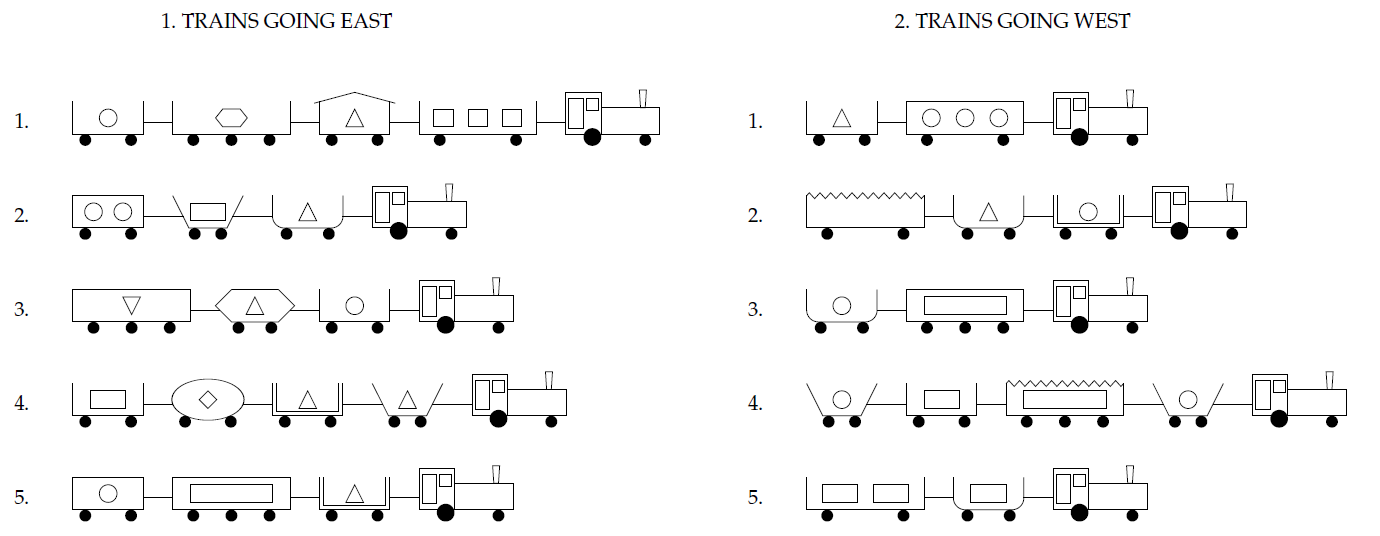
\includegraphics[width=0.9\linewidth]{michalskitrain.png}
        \caption{Trens de Michalski}
        \label{fig:trensmichalski}
    \end{figure}
    Em seguida, temos 10 variáveis booleanas (proposicionais) que indicam se cada par de tipos de carga está ou não em vagões adjacentes do trem. Além disso, também contamos com as seguintes relações entre os vagões de um trem, cujos valores lógicos variam entre 0 (Falso) e 1 (Verdadeiro):
    \begin{enumerate}
        \item Existe um retângulo próximo a um retângulo (V ou F);
        \item Existe um retângulo próximo a um triângulo (V ou F);
        \item Existe um retângulo próximo a um hexágono (V ou F);
        \item Existe um retângulo próximo a um círculo (V ou F);
        \item Existe um triângulo próximo a um triângulo (V ou F);
        \item Existe um triângulo próximo a um hexágono (V ou F);
        \item Existe um triângulo próximo a um círculo (V ou F);
        \item Existe um círculo próximo a um círculo (V ou F).
    \end{enumerate}

Existe um atributo de classe que define a direção do trem: leste ou oeste. Observe que para atributos com múltiplos valores, você deve atribuir valores na ordem em que eles aparecem. Por exemplo, o tipo de carga deve ser 1 para círculo, 2 para hexágono, 3 para retângulo e assim por diante.

O neurônio correspondente deve usar uma função linear, ou seja, $h(x) = x$.

Este problema tornou-se um padrão em testes e demonstrações de diversas técnicas de aprendizado de máquina, especialmente em implementações de indução lógica.

\section{Modelos utilizados}
Os modelos utilizados para a realização dos experimentos foram baseados no livro \textit{Neural-symbolic Cognitive Reasoning} de \cite{garcez2002neural}. Esses modelos podem ser encontrados no link \url{https://github.com/CarlosARL/IAFINAL}, juntamente com as instruções para execução do experimento.

Primeiramente, realizamos um pre-processamento da base de dados rotulada manualmente 

\subsection{Modelo da questão 1}
A rede neural de camadas densas utilizada segue as instruções do enunciado e é representada na figura fornecida. A arquitetura do modelo consiste em uma camada densa com 37 neurônios de entrada (um pra cada coluna da base da dados \textit{trains-100-mod.csv}, disponível no GitHub) e 9 neurônios de saída com ativação linear, seguida por uma segunda camada densa com 9 neurônios de entrada e um neurônio de saída, com ativação sigmoide. O neurônio de saída é responsável por classificar uma instância como leste (eastbound) ou oeste (westbound). A representação gráfica do modelo é mostrada na Figura \ref{fig:model1summary}.

\begin{figure}[H]
    \centering
    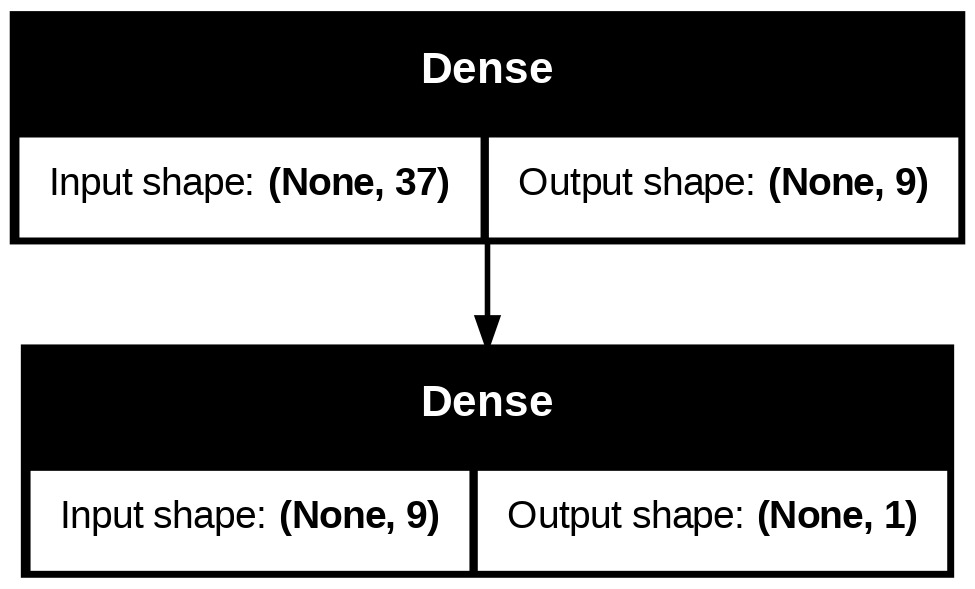
\includegraphics[width=0.5\linewidth]{model1summary.jpg}
    \caption{Modelo de camadas densas}
    \label{fig:model1summary}
\end{figure}

\subsection{Modelo da Questão 2 e Data Augmentation}

Para a segunda questão, optamos por utilizar uma meta-rede, composta por duas redes neurais que representam proposições. A camada final da meta-rede é responsável pela classificação final do problema. No cerne da meta-rede, implementamos 11 regras, cada uma equivalente a uma rede neural individual. As regras foram definidas da seguinte forma:

\begin{itemize}
    \item \textbf{num\_cars (t,nc):} Determina se o trem 't' $\in$ [1..10] possui 'nc' vagões, onde 'nc' varia entre 3 e 5.
    \item \textbf{loads(t,nl):} Verifica se o trem 't' $\in$ [1..10] possui 'nl' tipos de carga distintos, com 'nl' $\in$ [1..4].
    \item \textbf{wheels(t,c,w):}  Indica se o vagão 'c' $\in$ [1..4] do trem 't' $\in$ [1..10] possui 'w' rodas, onde 'w' pode ser 2 ou 3.
    \item \textbf{length(t,c,l):} Representa o comprimento do vagão 'c' $\in$ [1..4] do trem 't' $\in$ [1..10] como 'l', um vetor em \([-1, 1]^6\). 
    \item \textbf{shape(t,c,s):} Codifica a forma do vagão 'c' $\in$ [1..4] do trem 't' $\in$ [1..10] como 's', um vetor em \([1..10]^7\).
    \item \textbf{num\_car\_loads(t,c,ncl):}  Indica a quantidade de cargas 'ncl' $\in$ [0..3] no vagão 'c' $\in$ [1..4] do trem 't' $\in$ [1..10].
    \item \textbf{load\_shape(t,c,ls):}  Representa a forma da carga no vagão 'c' $\in$ [1..4] do trem 't' $\in$ [1..10] como 'ls' $\in$ [1..4].
    \item \textbf{next\_crc(t,c,x):}  Verifica se o vagão 'c' $\in$ [1..4] do trem 't' $\in$ [1..10] está adjacente a um vagão com carga circular. 'x' é um vetor booleano de tamanho 8.
    \item \textbf{next\_hex(t,c,x):}  Verifica se o vagão 'c' $\in$ [1..4] do trem 't' $\in$ [1..10] está adjacente a um vagão com carga hexagonal. 'x' é um vetor booleano de tamanho 8.
    \item \textbf{next\_rec(t,c,x):}  Verifica se o vagão 'c' $\in$ [1..4] do trem 't' $\in$ [1..10] está adjacente a um vagão com carga retangular. 'x' é um valor booleano.
    \item \textbf{next\_tri(t,c,x):}  Verifica se o vagão 'c' $\in$ [1..4] do trem 't' $\in$ [1..10] está adjacente a um vagão com carga triangular. 'x' é um vetor booleano de tamanho 8.
\end{itemize}

O treinamento da meta-rede foi realizado utilizando o método leave-one-out, onde um trem é selecionado para validação e os demais para treinamento. Para melhorar a capacidade de generalização do modelo, especialmente considerando o conjunto de dados limitado (10 trens), aplicamos uma técnica de aumento de dados (Data Augmentation). 

A técnica de Data Augmentation utilizada consiste em tratar cada vagão de um trem como uma instância independente durante o treinamento. Em outras palavras, se um trem possui 4 vagões, ele será considerado como 4 instâncias distintas no processo de treinamento, cada uma com suas características específicas. Com isso, o conjunto de dados original, composto por 10 trens, é expandido para 40 instâncias, aumentando a diversidade e representatividade dos dados para o treinamento da meta-rede.

A aplicação do Data Augmentation visa permitir que a meta-rede aprenda padrões não apenas em nível de trem completo, mas também em nível de vagão individual. Essa granularidade no aprendizado pode levar a um modelo mais robusto e capaz de generalizar melhor para novos dados, mesmo com um conjunto de dados inicial limitado.

Com o aumento de dados, a meta-rede foi treinada com 36 exemplos e validada com 4. A validação cruzada foi utilizada em relação a cada trem, garantindo que o modelo fosse avaliado em diferentes cenários e evitando um viés na avaliação do desempenho.

\begin{figure}[h]
    \centering
    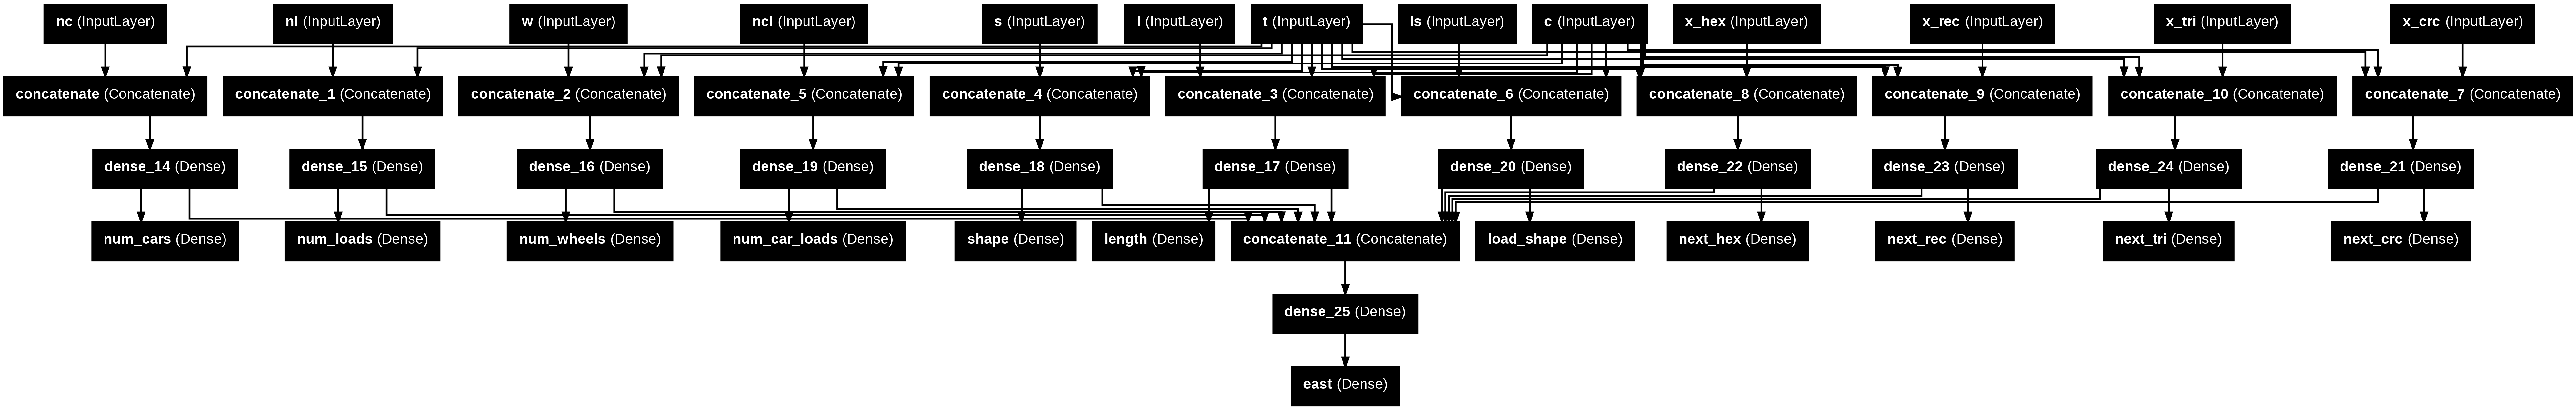
\includegraphics[width=1\linewidth]{metanet2.png}
    \caption{Metanet 2.}
    \label{fig:metanet2}
\end{figure}

\section{Resultados}

Nesta seção, discutiremos os resultados dos modelos descritos na seção anterior.

\subsection{Resultados do modelo da questão 1A}

Os gráficos apresentados na Figura \ref{fig:model1ACMGraphs} mostram as curvas de perda e acurácia durante o treinamento e teste do modelo, utilizando uma divisão de dados de 70/30 para treino e teste, respectivamente.

O gráfico à esquerda na Figura \ref{fig:model1ACMGraphs} exibe a perda do modelo ao longo das épocas. Observa-se uma diminuição contínua da perda tanto para o conjunto de treinamento quanto para o conjunto de teste. No início do treinamento, a perda é elevada para ambos os conjuntos, mas diminui rapidamente nas primeiras 50 épocas. A partir daí, a redução na perda continua, mas em um ritmo mais lento, até se estabilizar nas últimas épocas, parando o treinamento em torno de 250 épocas por meio de um \textit{EarlyStopping} definido no treinamento.

O gráfico à direita da Figura \ref{fig:model1ACMGraphs} mostra a acurácia do modelo ao longo das épocas. A acurácia do conjunto de treinamento aumenta de forma constante, atingindo um valor próximo de 70\% nas últimas épocas. A acurácia do conjunto de teste também aumenta, mas apresenta mais flutuações ao longo do treinamento, estabilizando-se em torno de 67\% nas últimas épocas, como mostrado também pela matriz de confusão da Figura \ref{fig:model1ACM}.

\begin{figure}[h]
    \centering
    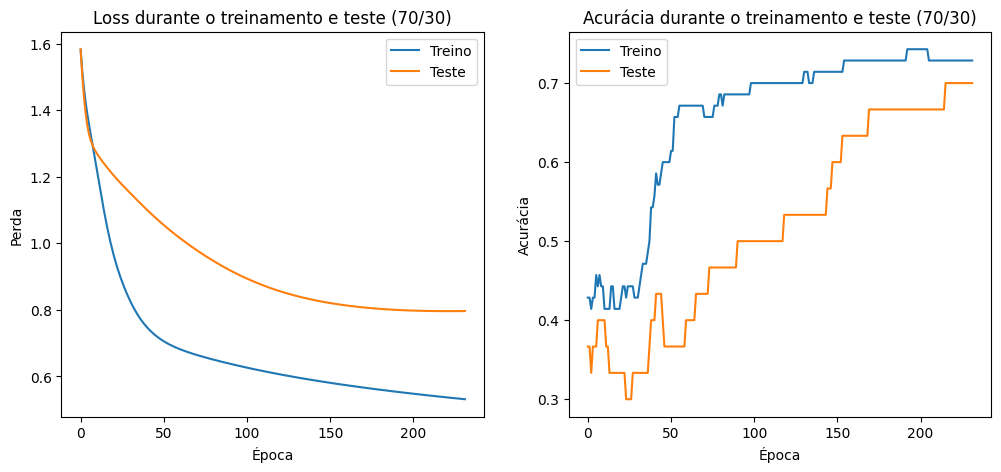
\includegraphics[width=1\linewidth]{casoA1.jpg}
    \caption{Gráficos de Loss e Acurácia durante o treino do caso A.}
    \label{fig:model1ACMGraphs}
\end{figure}

\begin{figure}[h]
    \centering
    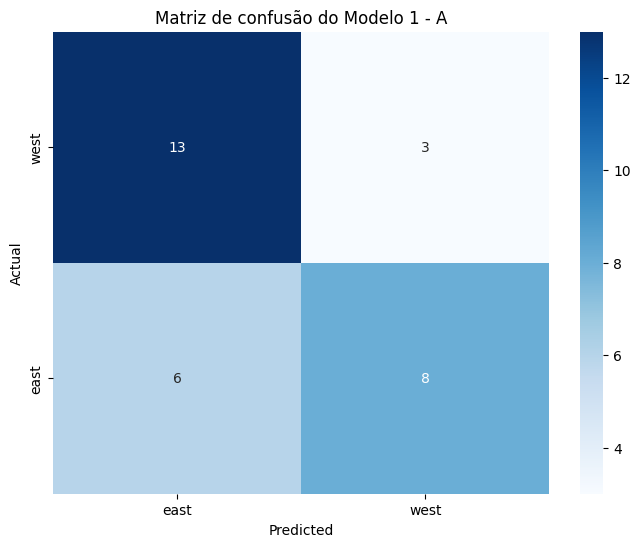
\includegraphics[width=0.7\linewidth]{cm1A.png}
    \caption{Matriz de confusão do teste do modelo 1 A.}
    \label{fig:model1ACM}
\end{figure}

\subsection{Resultados do modelo da questão 1B}

Os gráficos apresentados na Figura \ref{fig:model1BGraphs} mostram as curvas de perda e acurácia durante o processo de validação cruzada \textit{5-fold}, em que 5 \textit{folds}, cada um com divisão 80/20 para treinamento e teste, foram usados a fim de fazer a validação cruzada do modelo.

No primeiro par de gráficos, mostrado na Figura \ref{fig:model1Bfold}, o gráfico à esquerda exibe a perda por fold ao longo dos folds de validação cruzada. A linha azul representa a perda para cada fold, enquanto a linha vermelha pontilhada indica a média da perda ao longo dos folds, e a área sombreada em rosa representa o desvio padrão da perda. Observa-se que a perda varia entre os folds, com a média situando-se em torno de 70\%.

O gráfico à direita desse mesmo par mostra a acurácia por fold ao longo dos folds. A linha azul indica a acurácia para cada fold, a linha vermelha pontilhada representa a média da acurácia, e a área sombreada em rosa indica o desvio padrão da acurácia. Nota-se que a acurácia flutua entre os folds, com uma média próxima de 57.5\%, e o desvio padrão reflete a variabilidade entre as diferentes iterações.

No segundo par de gráficos, mostrados na Figura \ref{fig:model1BGraphs}, o gráfico à esquerda mostra a perda durante o treinamento ao longo das épocas para cada fold. Cada cor representa um fold diferente, e observa-se uma diminuição contínua da perda, que é mais acentuada nas primeiras épocas e vai se estabilizando ao longo do tempo, sendo este comportamento comum a todos os folds. O EarlyStopping é aplicado para interromper o treinamento quando a perda se estabiliza, prevenindo overfitting, e observa-se que o Fold 5 foi o que mais treinou, parando apenas depois de centésima época.

O gráfico à direita desse mesmo par exibe a acurácia durante o treinamento ao longo das épocas para cada fold. Assim como no gráfico de perda, cada cor corresponde a um fold diferente. A acurácia aumenta de forma constante durante o treinamento, estabilizando-se ao longo das épocas em torno de 70\% para todos os folds.

\begin{figure}[H]
    \centering
    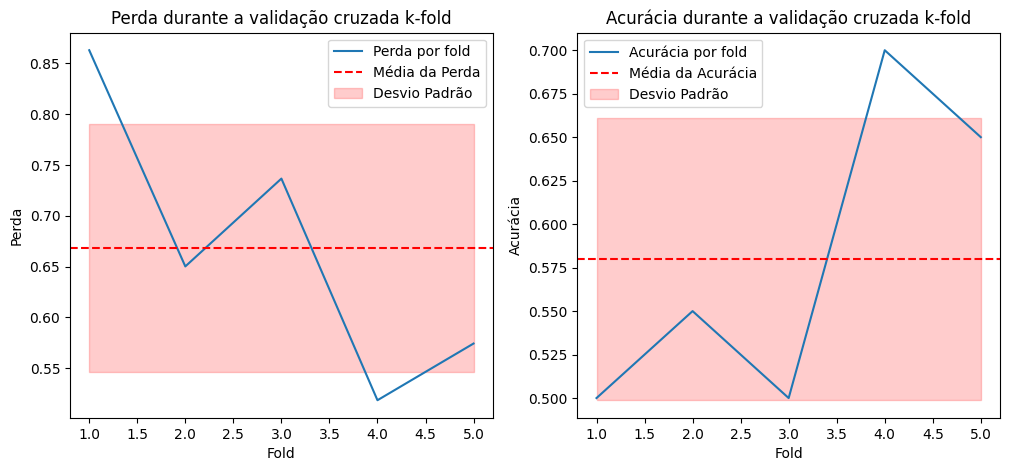
\includegraphics[width=1\linewidth]{casoB1folds.png}
    \caption{Perda e acurácia por fold no modelo B da questão 1.}
    \label{fig:model1Bfold}
\end{figure}

\begin{figure}[H]
    \centering
    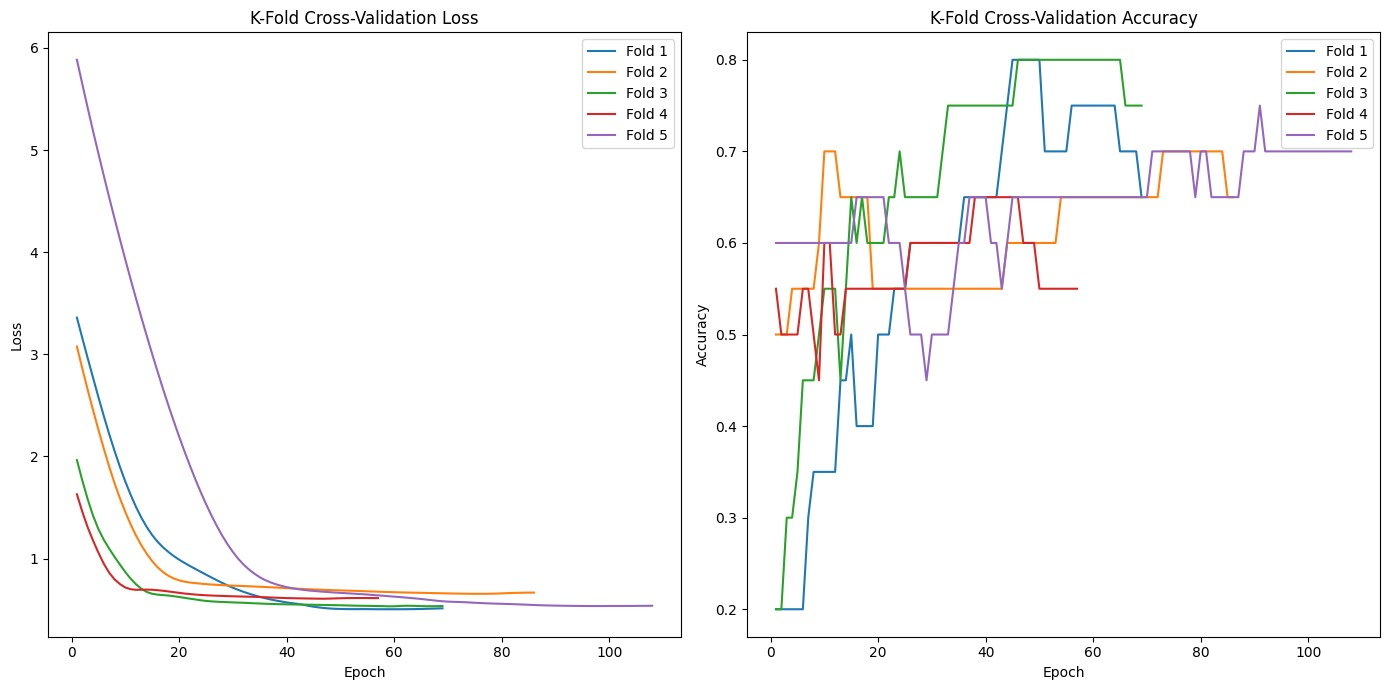
\includegraphics[width=1\linewidth]{casoB1.png}
    \caption{Perda e acurácia por época no modelo B da questão 1.}
    \label{fig:model1BGraphs}
\end{figure}

\subsection{Resultados do modelo da questão 2}

Os gráficos nas Figuras \ref{fig:model2bacc} e \ref{fig:model2Amse} mostram as curvas de perda e acurácia durante o treinamento e teste do modelo, utilizando o método LeaveOneOut de validação cruzada para treino e teste do modelo descrito.

O gráfico da Figura \ref{fig:model2bacc} exibe a acurácia binária do modelo ao longo das épocas. Observa-se que a acurácia do conjunto de validação (val) é muito alta desde o início, atingindo rapidamente o valor de 1.0. Já a acurácia do conjunto de treinamento (train) apresenta um comportamento mais instável no começo, mas se estabiliza em torno de 0.6 após as primeiras 50 épocas.

\begin{figure}[h]
    \centering
    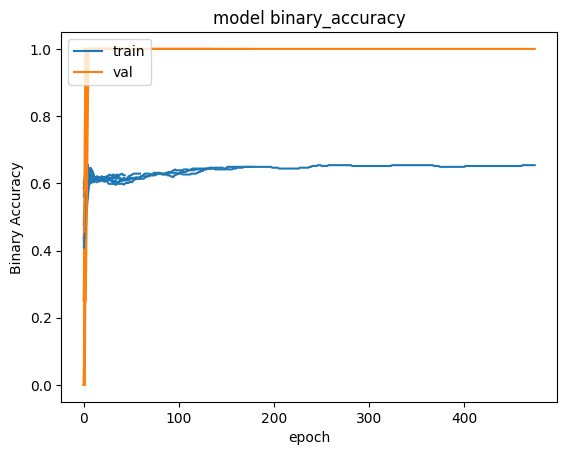
\includegraphics[width=0.8\linewidth]{bacc.png}
    \caption{Perda e acurácia por época no modelo B da questão 1.}
    \label{fig:model2bacc}
\end{figure}

O gráfico à direita da Figura \ref{fig:model2Amse} mostra o erro quadrático médio (MSE) do modelo ao longo das épocas. Inicialmente, o MSE é alto para ambos os conjuntos de dados, mas diminui rapidamente nas primeiras 50 épocas. A partir daí, o MSE para o conjunto de validação continua a diminuir até quase zero, enquanto o MSE do conjunto de treinamento se estabiliza em torno de 0.2.

\begin{figure}[h]
    \centering
    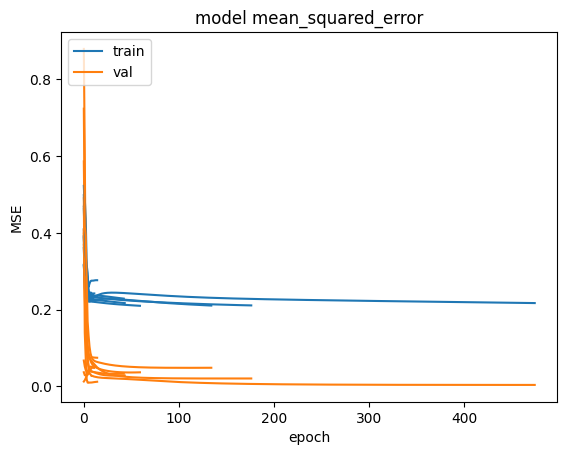
\includegraphics[width=0.8\linewidth]{MSE.png}
    \caption{Perda e acurácia por época no modelo B da questão 1.}
    \label{fig:model2Amse}
\end{figure}


\subsection{Resultados dos testes para a questão 3}

\subsubsection{Letra A}

Nesta seção, discutiremos os resultados da questão 3.
Na letra A, os modelos utilizados nas questões 1 e 2 apresentam diferenças significativas em suas arquiteturas, o que resulta em variações nos resultados numéricos. Na Questão 1, foi utilizado um modelo neuro-simbólico adaptado para classificar trens com base em predicados lógicos. Este modelo combina aprendizagem simbólica com redes neurais, utilizando predicados lógicos e as relações entre estes atributos para inferir a direção dos trens. A abordagem neuro-simbólica tende a ser mais interpretável devido aos componentes simbólicos que permitem uma compreensão mais direta das inferências feitas pelo modelo.

Por outro lado, na Questão 2, foi implementada uma solução utilizando LTNTorch, que integra a lógica simbólica diretamente na arquitetura da rede neural. O LTNTorch usa técnicas de aprendizado profundo para ajustar os pesos da rede neural, otimizando uma função de custo que incorpora restrições lógicas. Essa abordagem combina o poder de representação das redes neurais com as capacidades interpretativas da lógica simbólica. A integração profunda da lógica na rede neural permite que o modelo LTNTorch capture relações mais complexas nos dados, o que pode levar a uma melhor generalização dos resultados.\\
Nos resultados numéricos, o modelo LTNTorch tende a apresentar uma performance superior, especialmente em cenários que requerem a modelagem de relações complexas. A capacidade das redes neurais profundas de aprender representações complexas dos dados confere ao LTNTorch uma vantagem em termos de precisão e generalização. Por outro lado, o modelo neuro-simbólico, embora melhor interpretável, pode enfrentar limitações ao lidar com relações complexas que são mais facilmente capturadas por redes neurais profundas.

\subsubsection{Letra B}

Para extrair a regra genérica $\text{car}(T,C) \land \text{short}(C) \land \text{closed\_top}(C) \rightarrow \text{east}(T)$ dos dois modelos, o algoritmo de extração de conhecimento descrito no material de classe é útil para o propósito. A extração de regras de um modelo treinado envolve identificar padrões nas entradas e saídas que permitem derivar regras simbólicas.

Primeiramente, abordamos o processo de extração com base nos princípios gerais discutidos no material \textit{Symbolic Knowledge Extraction from Trained Neural Networks} por \cite{DAVILAGARCEZ2001155} O processo de extração pode ser dividido em etapas distintas, começando pela identificação dos conceitos. Cada neurônio na camada de entrada representa uma característica dos dados (como $\text{car}$, $\text{short}$, e $\text{closed\_top}$), enquanto a camada de saída representa a classe ou rótulo predito, que neste caso é $\text{east}$.

A seguir, o conhecimento adquirido pela rede neural durante o treinamento é codificado na arquitetura da rede, na função de ativação associada e nos valores dos pesos. Para extrair o conhecimento, devemos interpretar a combinação desses elementos de forma compreensível. Assim, definimos as regras de extração, que consistem em mapear as entradas diretamente nas saídas da rede. Utilizamos uma abordagem decomposicional onde analisamos as ativações individuais dos neurônios na camada intermediária e como eles contribuem para a ativação do neurônio de saída.

\subsubsection{Letra C}
Na letra C, três casos de verificação de aprendizado das redes foram apresentados, sendo eles:

\begin{itemize}
    \item Se um trem tem um vagão curto e fechado, então ele vai para o leste, caso
contrário, vai para o oeste.
    \item Se um trem tem dois vagões, ou tem um vagão com teto irregular, então ele
vai para o oeste, caso contrário, vai para o leste.
    \item Se um trem tiver mais de dois tipos diferentes de carga, então ele vai para o
leste, caso contrário, vai para o oeste
\end{itemize}

Para averiguar os itens definidos, criamos dados de trens com e sem as características descritas em cada um dos casos, e os resultados podem ser vistos nas Figuras \ref{fig:ca}, \ref{fig:cb} e \ref{fig:cc}.

\begin{figure}[H]
    \centering
    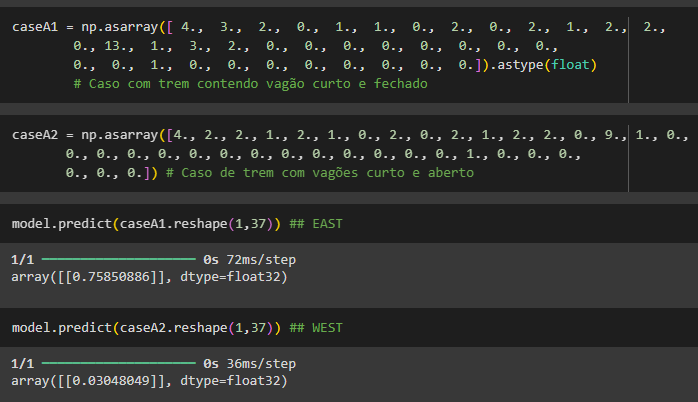
\includegraphics[width=0.8\linewidth]{3CA.png}
    \caption{Testes para o caso A.}
    \label{fig:ca}
\end{figure}

\begin{figure}[H]
    \centering
    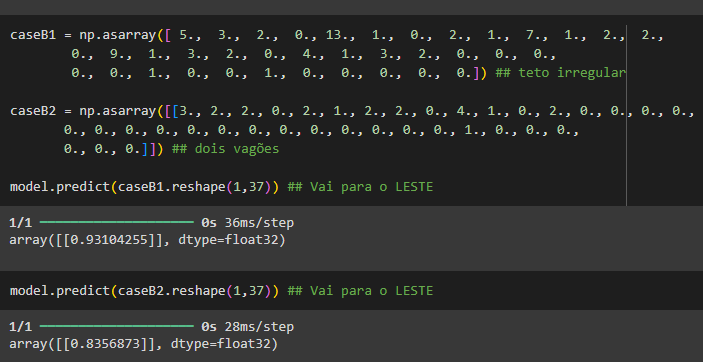
\includegraphics[width=0.8\linewidth]{3CB.png}
    \caption{Testes para o caso B.}
    \label{fig:cb}
\end{figure}

\begin{figure}[H]
    \centering
    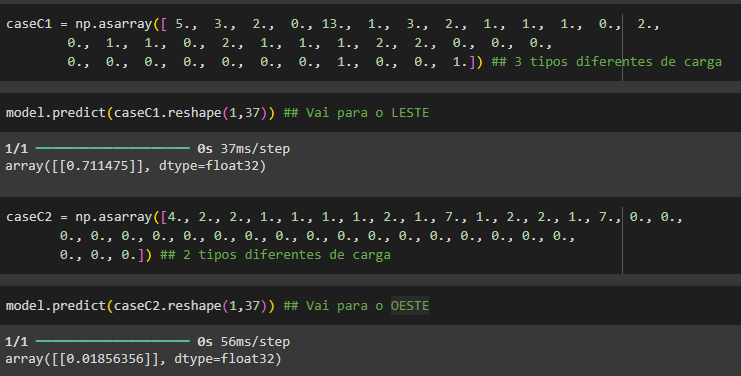
\includegraphics[width=0.8\linewidth]{3CC.png}
    \caption{Testes para o caso C.}
    \label{fig:cc}
\end{figure}

Na Figura \ref{fig:ca}, definimos o caso de um trem com vagão curto e fechado que foi guardado na variável casoA1, e outro trem que define um trem com vagão curto e aberto, guardado na variável casoA2. Neste caso, o modelo definiu que o trem casoA1 está indo para leste, enquanto o trem casoA2 está indo para oeste. 

Na Figura \ref{fig:cb}, definimos o caso de um trem com vagão com teto irregular que foi guardado na variável casoB1, e outro trem que define um trem que possui apenas dois vagões de carga, guardado na variável casoB2. Neste caso, o modelo definiu que tanto o trem casoB1 quanto o trem casoB2 estão indo para leste, confirmando a tese definida na questão.

Na Figura \ref{fig:cc}, definimos o caso de um trem que carrega mais de dois tipos diferentes de carga (index 1 do array) que foi guardado na variável casoC1, e outro trem que possui exatamente dois tipos de carga, guardado na variável casoC2. Neste caso, o modelo definiu que o trem casoC1 vai para leste, enquanto o trem casoC2 vai para oeste.

\bibliographystyle{sbc}
\bibliography{sbc-template}

\end{document}